\documentclass[a4paper]{article}
\usepackage{geometry}
\usepackage[utf8]{inputenc}
\usepackage[T1]{fontenc}
\usepackage[bookmarks,colorlinks]{hyperref}
\usepackage[french]{babel}
\usepackage{pdflscape}
\usepackage{graphicx}

\title{Rapport d'analyse du projet de Technologies Objets}
\author{Maxime Arthaud \and Korantin Auguste \and Martin Carton}
\date{24 Mai 2013}

\begin{document}
\maketitle

\section{Scénarios d'utilisation}
  Notre raytracer sera utilisé pour créer des images à partir de scènes 3D décrites
  dans des fichiers.
  Nous fournirons aussi un petit utilitaire pour créer ces fichiers décrivant des scènes.

\section{Démarche}
  Nous avons commencé par faire la liste des choses à faire. Nous avons décidé
  de séparer l'interface graphique de la partie génération d'image. L'interface
  graphique permettra de générer un fichier contenant toutes les informations
  nécessaires à la génération de l'image qui sera faite par un second programme
  utilisable en ligne de commande, ce fichier sera simple et pourra être écrit
  à la main.

\section{Tâches effectuées}
  Nous avons commencé à réfléchir à l'organisation des classes, à l'interface
  utilisateur et au format de fichier.

  \subsection{Diagramme d'analyse}

    Nous avons décidé de structurer notre programme de la manière suivante :
    Tout d'abord, une classe va se charger de lire le fichier décrivant la scène,
    pour construire un objet scène en conséquence.

    Les objets que contiendra la scène devront tous contenir une méthode
    \verb+computeColor+, qui sera chargée de donner la couleur d'un rayon
    arrivant sur l'objet (et appellera récursivement cette même méthode pour
    d'autres objets, dans la plupart des cas).
    Une seconde méthode, \verb+distance+, est chargée de donner la distance parcourue
    le long du rayon passé en paramètre pour arriver jusqu'à l'objet. Elle renvoie « NaN »
    si le rayon n'intersecte pas l'objet.

    Un objet pourra soit être un « Mesh », composé de plusieurs triangles (ce sera le cas
    d'un cube), soit être un objet possédant tous les caractéristiques optiques nécessaires.

    Il sera donc très facile de générer notre image : Il suffira, pour chaque rayon commençant par
    le point de vue de l'observateur et passant par un pixel de l'écran, de trouver quel est le premier
    object qu'il intersecte grâce à la méthode \verb+distance+, et d'utiliser la méthode \verb+computeColor+
    pour calculer la couleur de ce point de l'objet.

    La figure \ref{fig:uml} présente les relations entre les différentes classes
    que nous envisageons d'utiliser.

  \subsection{Interface utilisateur}
    La figure \ref{fig:gui} présente l'interface graphique telle que nous
    envisageons de la faire.

    Les différents objets (caméra (c'est à dire point de vue et écran),
    sphères, cubes et plans) peuvent être y ajoutés selon leurs différentes
    propriétés optiques et supprimés. Un résumé des objets créés est affiché, on
    peut directement lancer la génération de l'image, ou enregistrer le fichier.

  %\subsection{Diagramme de séquence}
  \subsection{Format de fichier}
    Le fichier sera un fichier texte où chaque objet sera représenté sur une
    ligne. Chaque ligne sera de la forme
    \verb+Nom(nom1=valeur1, nom2=valeur2, .., nomN=valeurN)+ où \verb+Nom+ est
    le nom de l'objet à créer (Camera, Sphere, Cube ou Plane), et les noms et
    valeurs sont les données qui caractérisent l'objet, par exemple le rayon
    et le centre pour la Sphere, ou encore la réflectance.

    \newgeometry{width=1.3\linewidth}
    \begin{landscape}
      \thispagestyle{empty}
      \begin{figure}[p]
        \makebox[\paperwidth][c]{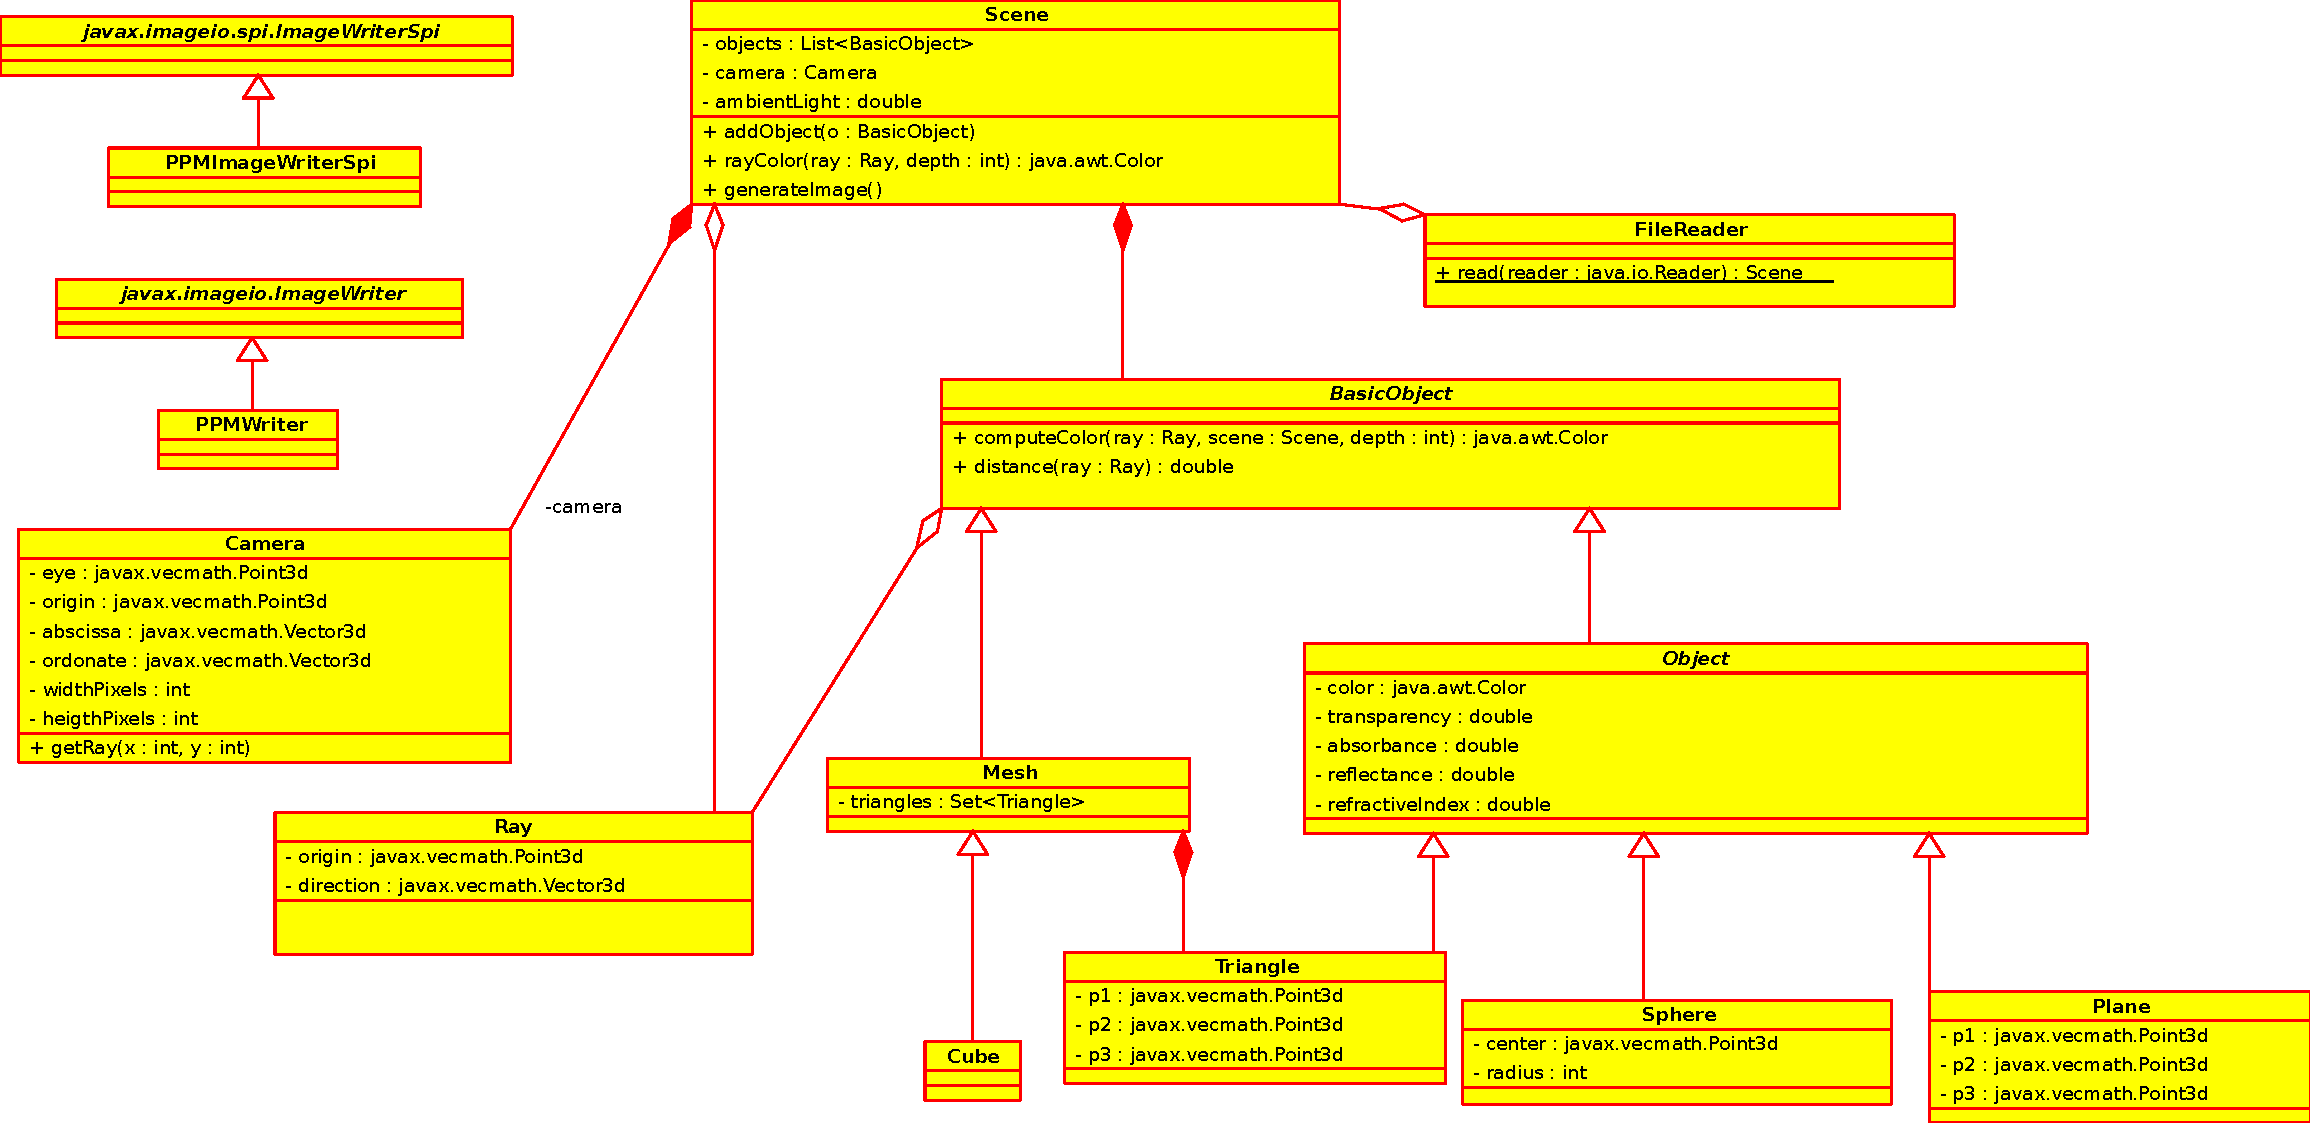
\includegraphics[width=26cm]{uml.pdf}}
        \caption{Diagramme UML\label{fig:uml}}
      \end{figure}
    \end{landscape}
    \restoregeometry

    \begin{figure}[p]
      \centerline{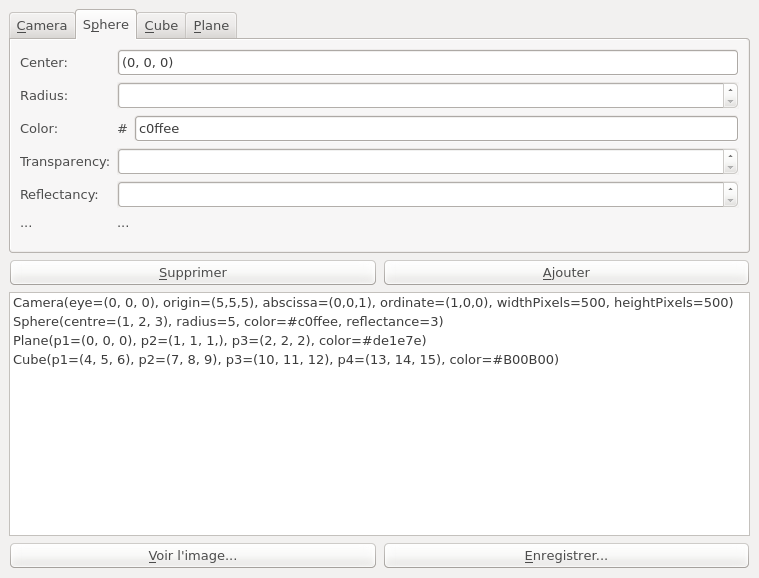
\includegraphics[width=1.2\textwidth]{gui.png}}
    \caption{Interface graphique\label{fig:gui}}
    \end{figure}

\end{document}

